\documentclass[uplatex,dvipdfmx,a4paper,twocolumn,base=11pt,jbase=11pt,ja=standard]{bxjsarticle}  % 環境に合わせて変更してください

\usepackage{ipsj}
\usepackage{color}

%追加パッケージ
\usepackage{enumerate}
\usepackage{url}
\usepackage[dvipdfmx]{graphicx}
%\usepackage{caption}

\newcommand{\todo}[1]{\colorbox{yellow}{{\bf TODO}:}{\color{red} {\textbf{[#1]}}}}

\title{発生頻度の少ないコーディング規約違反データ統合による\\検出精度向上への試み}{Toward improving detection accuracy by integrating occasional coding convention violations datasets}
\author{和歌山大学}{亀岡 令}{Ryo Kameoka, Wakayama University}
\author{和歌山大学}{伊原 彰紀}{Akinori Ihara, Wakayama University}
\author{和歌山大学}{南 雄太}{Yuta Minami, Wakayama University}
\author{和歌山大学}{大森 楓木}{Fuki Omori, Wakayama University}

\begin{document}
\maketitle

%================
%1
\section{はじめに}
%================
%hogehoge(背景,動機とか)
ソフトウェアを共同開発するプロジェクトでは,他者が実装したソースコードでも保守を容易にするために,コーディング規約を遵守する可読性の高いソースコードの実装が期待される.具体的には,PythonのPEP8やJavaのCode Conventions for the Java Programming Languageなど,各言語が標準的な規約を公開している.各プロジェクトは,保守性や可読性を高めるためにインデントや括弧などの記法\todo{記法だけだっけ?エラー,プログラムの特徴量(複雑度)なども含んでいなかった?}を標準的な規約に加えて個々に定めることもある.

%開発者は保守管理の観点から,コーディング規約を遵守することによって可読性の高いコードを書くことが求められる.コーディング規約とは,ソースコードを記述する際に,保守性や可読性を高めるためにインデントや括弧などの記法を定めたものである.コーディング規約の例として,PythonのPEP8やJavaのCode Conventions for the Java Programming Languageなどがある.ただし,開発者が自らこれらの規約に違反しているコード断片を特定し,修正を行うことは時間的コストを要するため,静的解析ツールツールが用いられる.

多くのプロジェクトでは静的解析ツールを用いることで規約を違反するソースコードの検出を自動化している.一方で,開発者は\todo{XXのため}静的解析ツールが検出する膨大な違反の中から,修正すべき違反の選択が余儀なくされる.従来研究では,機械学習を用いて優先的に修正すべき規約違反を推薦する手法を提案している~\cite{article1}.しかし,規約違反の種類ごとの発生頻度が低く,修正率\todo{発生率?}が低い規約は,推薦精度に影響する.特に,新規プロジェクトでは過去に発生した違反修正履歴を持たないため,規約違反の推薦は容易でない.


%静的解析ツールは,ツールによって定義されたルールによって該当するすべてのコーディング規約違反を検出することができる.これによってプログラム中のコーディング規約違反が大量に発見されることが多い.だが,開発者がここで発見された規約違反コードをすべて修正することは無い.従来研究では,機械学習を用いて静的解析ツールによって発見された規約違反が修正されたかを学習し,優先して修正すべき規約違反の検出を行っている~\cite{article1}.しかし,規約違反の種類ごとの分布には偏りがあるため,違反頻度の低い規約は機械学習において,予測精度は学習データセットの大きさ,正例不例の割合などに依存する問題が起こる.

%===============
本研究では,\todo{何のために?}連合学習を用いた\todo{何を?特にクロスプロジェクトのことを書くべきでは?}予測するモデルを提案する.連合学習は,学習データから得られたモデルに加えて,別の学習データから得られたモデルも利用してモデルを構築するため,それぞれの学習データセットの特徴を考慮することができる.\todo{だから何?}本研究では,プログラムの編集履歴を特徴量とし,違反が修正された編集の特徴をもとにし,連合学習によって構築されたモデルを利用することで,\todo{従来研究よりどのように良い方法であるのかを一言で書くべきでは?}規約違反が修正させるかを予測する.

%本研究では,連合学習を用いて学習することで,予測精度の向上させることを目的とする.連合学習は,学習データから得られたモデルに加えて,別の学習データから得られたモデルも利用してモデルを構築するため,それぞれの学習データセットの特徴を考慮することができる.具体的には,プログラムの編集履歴を特徴量とし,違反が修正された編集の特徴をもとにし,連合学習によって構築されたモデルを利用することで,規約違反が修正させるかを予測する.
%================
%2
\section{分析}
%================


%================
%hogehoge(どんなデータセット使ったか)

%fugofugo(そこからどんなデータをどうやって集めたか)

%2.1の修正版



%================
%2.2
\subsection{データセット}
本研究では,GitHubからPythonで実装されておりPylintを用いて開発しているtransitions, schematics, schema\_salad, python-bugzilla, python-cloudant, pyscard, pynput, OWSLib, howdoi, hickleの10リポジトリを対象とする.これらのリポジトリからそれぞれ1,000日間のコミット(\todo{中央値でXXコミット分})を分析対象とする.

\subsection{分析手法}
規約違反が修正されるかの予測には,\todo{従来研究で使用された??}変更行数や複雑度などソースコードや編集についての43個の特徴量を抽出し,FedAvgアルゴリズムを用いた連合学習を行う~\cite{article2}.目的変数は,ある\todo{「ある」とは?}コミットにおいて規約違反が修正有無の2クラス分類とし,説明変数には規約違反の種類やソースコードの複雑度などの44個\todo{上の43ではない?}のパラメータを用いる.\todo{規約違反検出数に対して修正された違反数が極端に少ないため?}学習データとテストデータは,コミットの古い順から7割を学習データとし,残り3割を予測データとすることで,時系列を考慮した予測を行う.

図1は,FedAvgを用いた連合学習の概要を示し,個別\todo{この研究ではプロジェクトごとってこと?}の深層学習によって得られたモデルを集約し平均を取り,再度学習する際に出力されたモデルと,先ほど\todo{先ほどとは?}得られたモデルとの平均\todo{中央値ではなく?普通は平均を使うものなの?}とする.モデルの構築,得られたモデルの集約,再度学習を繰り返すことで,より精度の高いモデルを得る手法である.実装には,オープンソースフレームワークのOpenFLを用いる.

本論文で使用するFebAvgにおいて,深層学習のレイヤーは3層で,1,2層目はReLU層であり,3層目にシグモイド関数を用いた出力層となっている.最適化アルゴリズムにはAdamを利用し,学習率は0.01に設定した.

%===============
%FLの説明用図
%===============
%\begin{figure}[t]
%  \centering
%  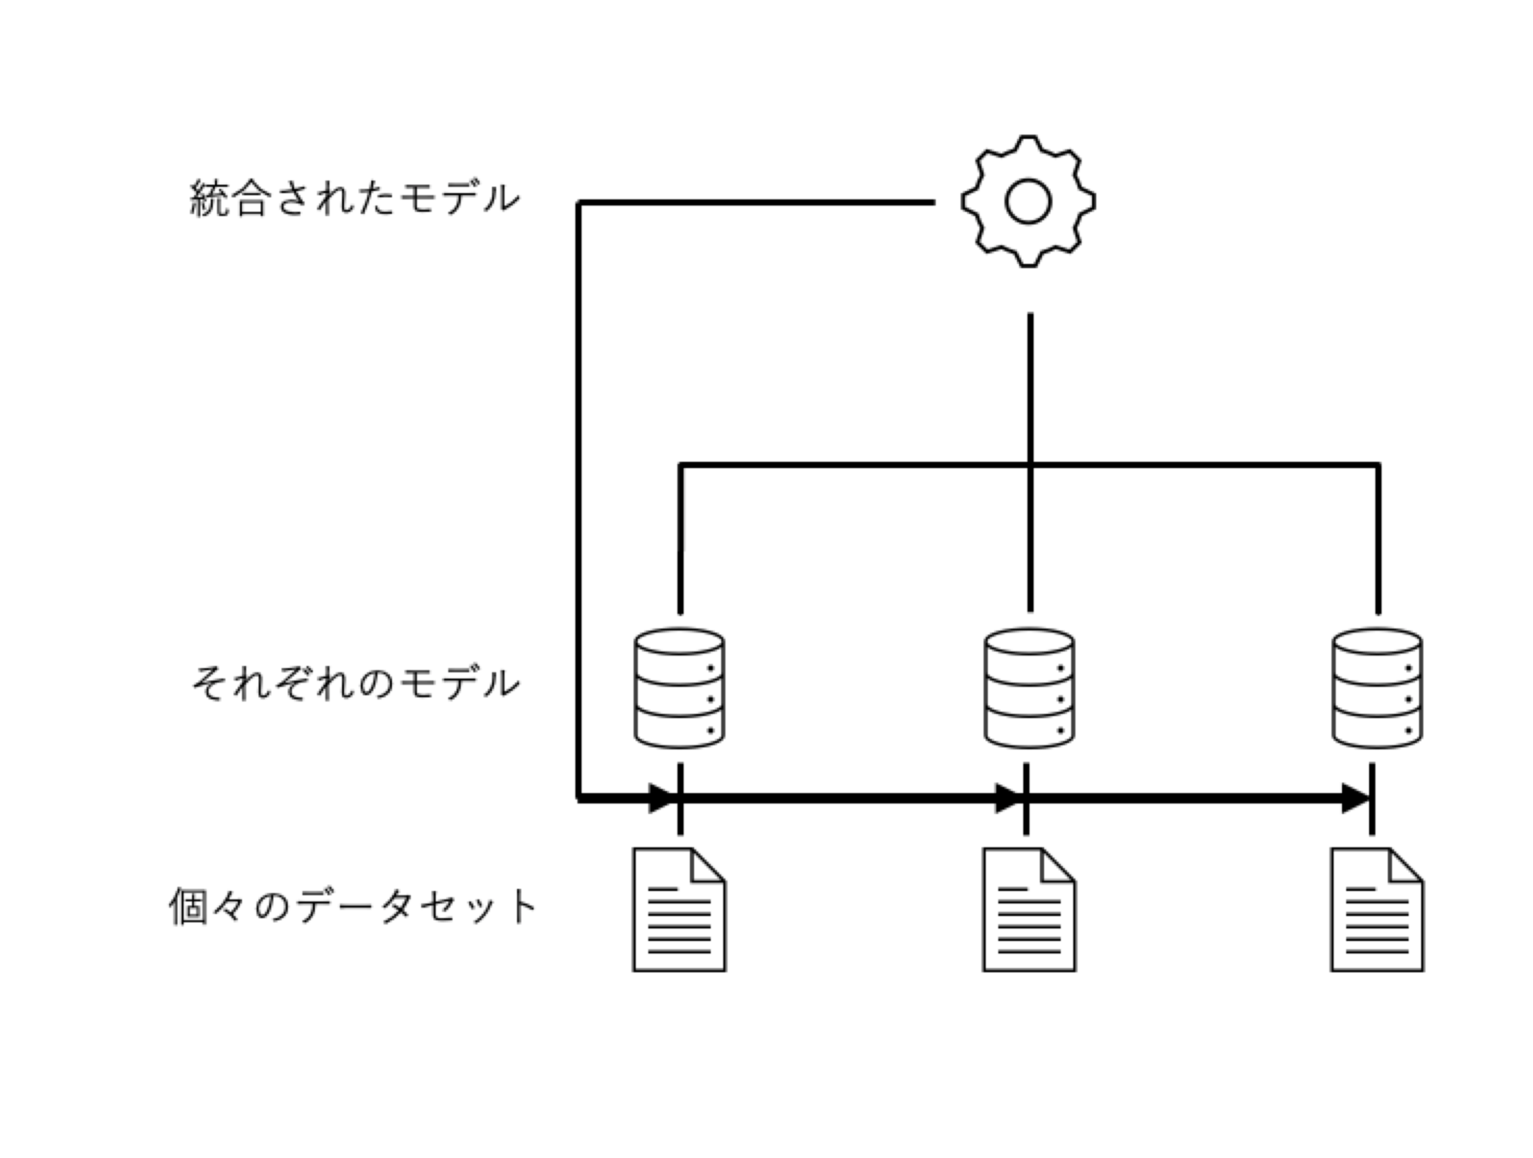
\includegraphics[width=6.5cm]{federated_learning_exp.pdf} 
%  \caption{連合学習}
%  \label{fig:test}
%  \end{figure}

%\begin{figure}[t]
%	\centering
%	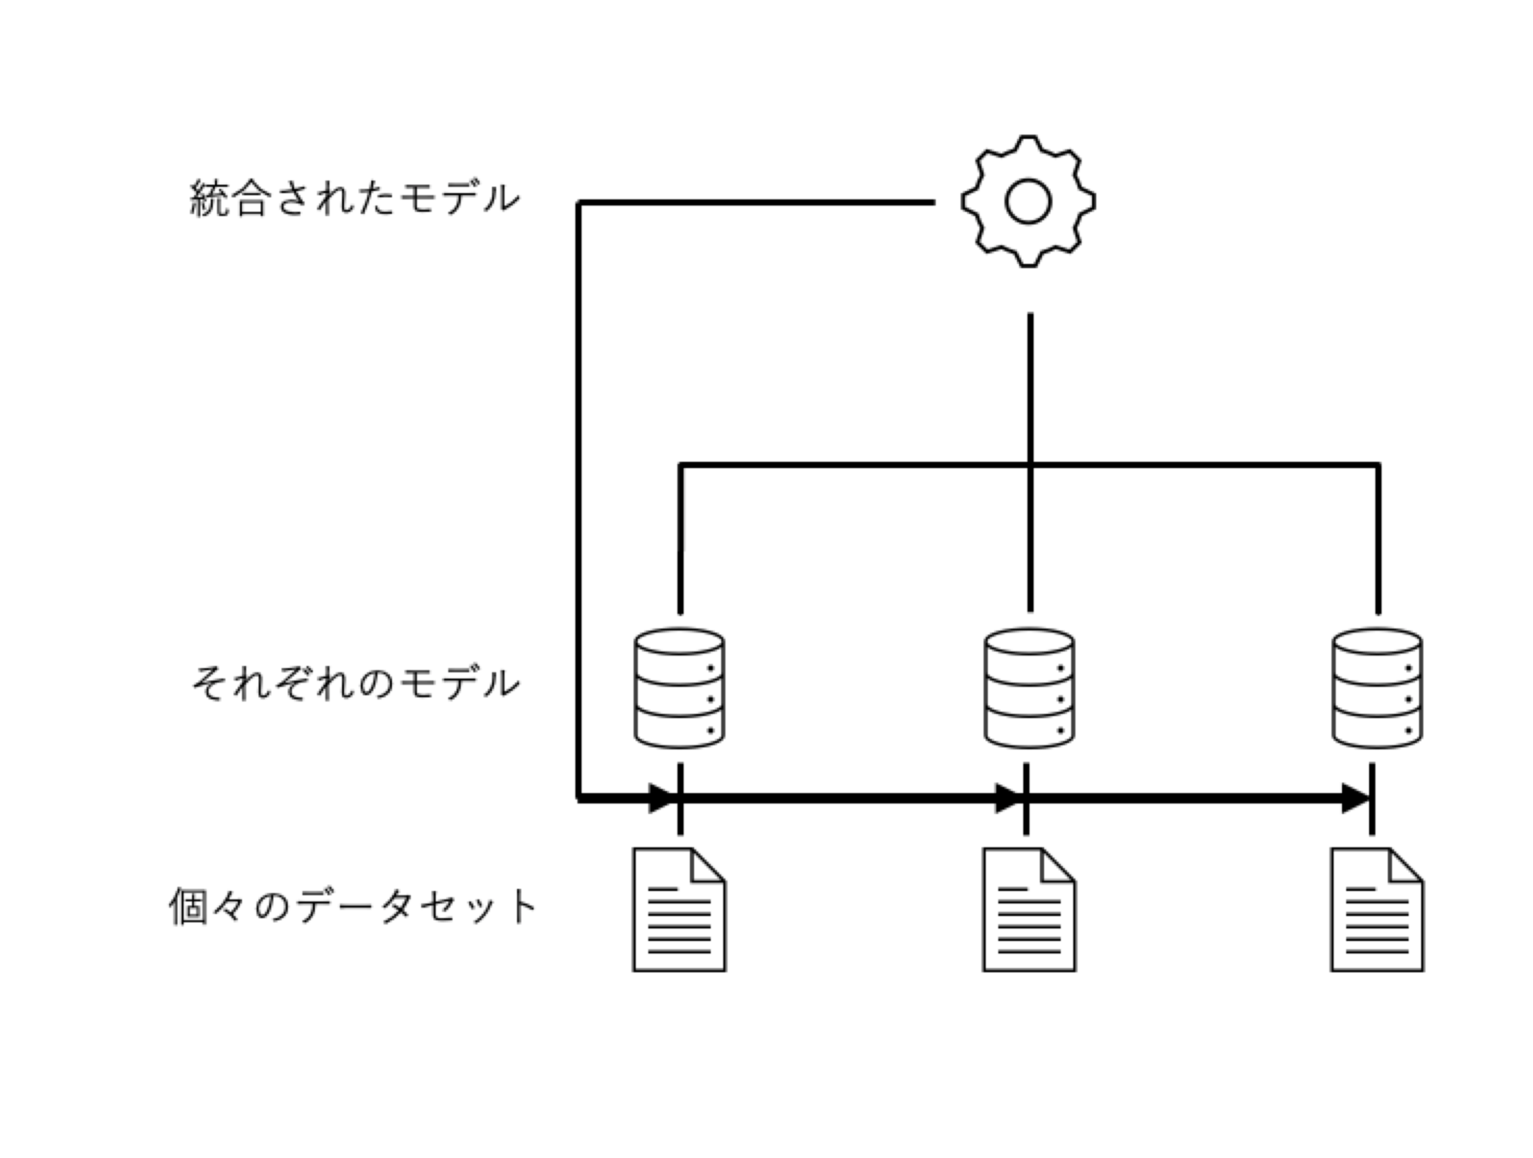
\includegraphics[width=1.0\linewidth]{federated_learning_exp.pdf}
%	\caption{連合学習の概略図}
%	\label{fig:test}
%\end{figure}

%-----------
\begin{figure}
\begin{center}
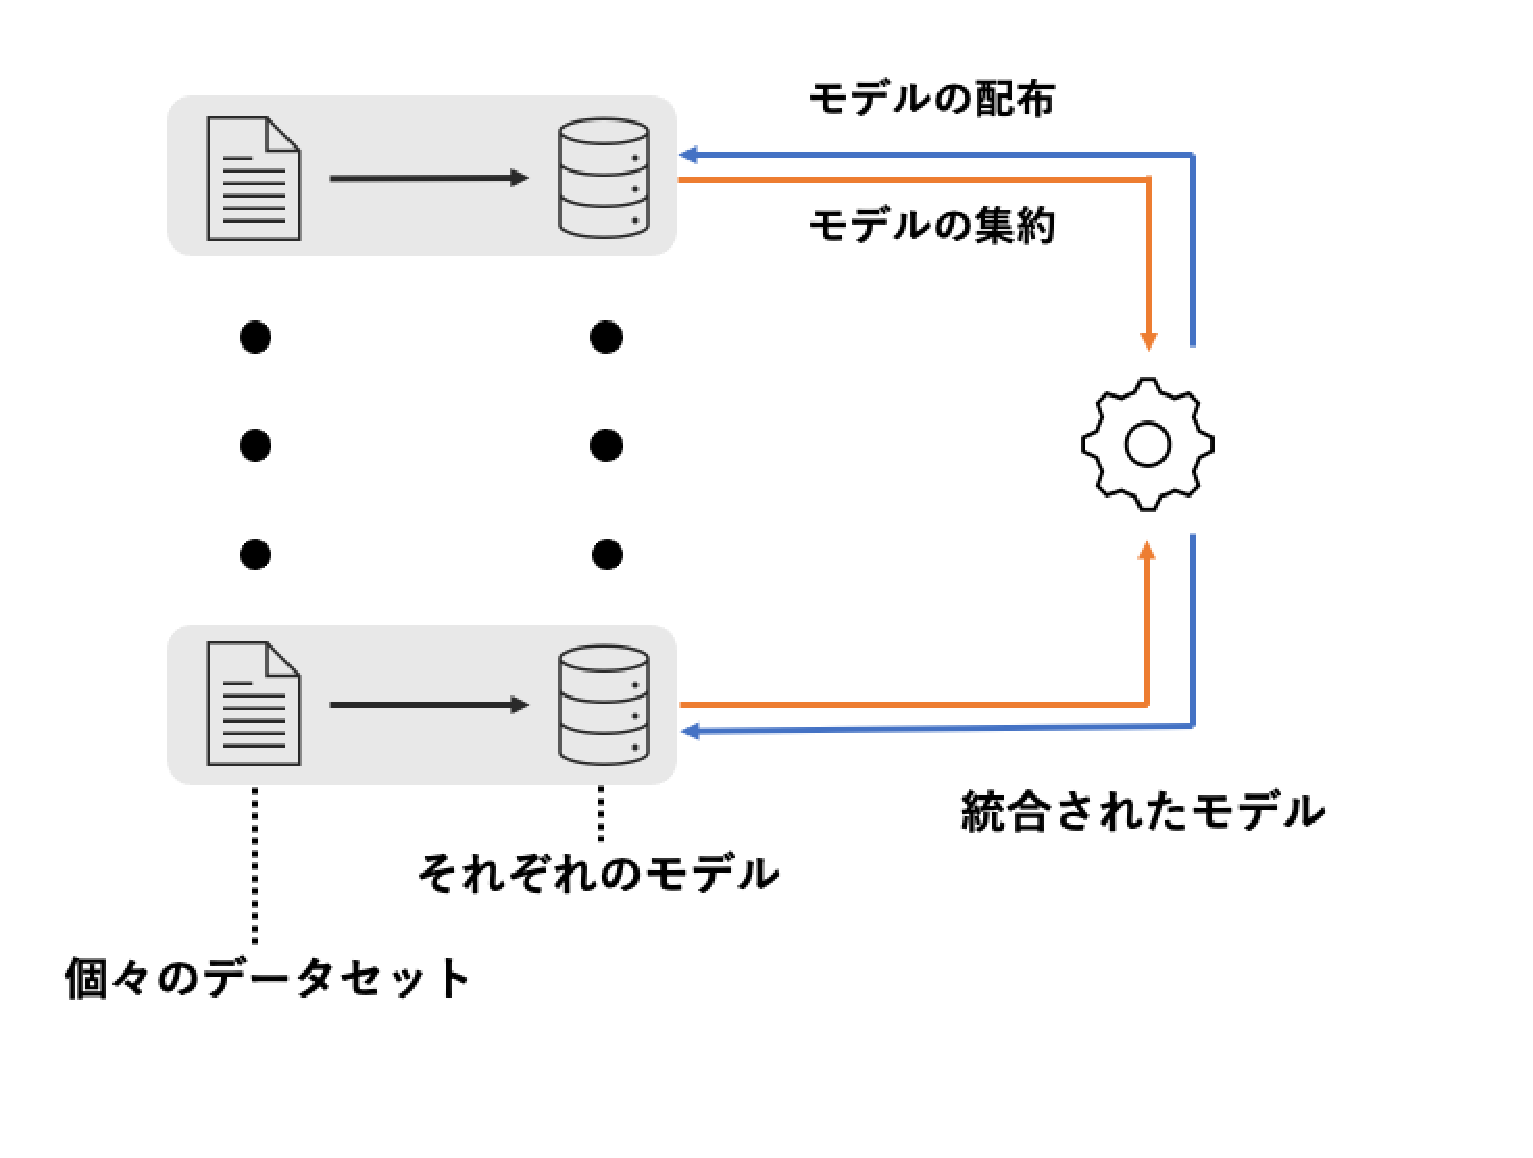
\includegraphics[width=0.9\linewidth]{federated_learning_exp.eps}
\caption{連合学習の概略図}
\label{fig:test}
\end{center}
\end{figure}
%-----------


%================
%結果の表

\begin{table}[t]
\vspace{0mm}
 \centering
 \caption{分析結果}
\label{tab:result3}
  \scalebox{1.0}{
  \begin{tabular}{l|r|r|r} \hline
    & \multicolumn{1}{c|}{適合率} & \multicolumn{1}{c|}{再現率} & \multicolumn{1}{c}{F1値} \\ \hline
    連合学習モデル & 0.03 & 0.52 & 0.06 \\ \hline
    深層学習モデル & 0.03 & 0.32 & 0.05 \\ \hline
  \end{tabular}
    \label{tab:result1}
   }
\end{table}

%連合学習(over)
% 正解率: 0.613
% 適合率:  0.034
% 再現率:  0.523
% F1値:  0.063

%連合学習(under)
% 適合率:  0.03799660941991597
% 再現率:  0.28169398907103826
% F1値:  0.06696109631746444

%深層学習(over)
% 適合率:  0.02880505941352306
% 再現率:  0.3185792349726776
% F1値:  0.052833095448469605
%================
%2.4
\subsection{結果}
分析の結果から~~~~~

%================
%hogehoge(どんな結果が得られたか,図とかを一緒に載せる)

%fugofugo(結果からの考察)
%分析を行った結果次のような結果が得られた.

%--------------------------------表入れるとこ



%================
%3
\section{おわりに}

本研究では,静的解析ツールによって検出された規約違反が予測地点において修正されるかを, 連合学習によって精度向上を試みた.今後の方針として,データセットの拡張,違反頻度の低い規約違反への重み付けなどを用いて予測精度の高いモデルの構築を目指す.
%================

%hogehoge(今回の研究のまとめとか)

%fugofugo(今回研究から得られたことを踏まえて今後どう発展させていくか)

%42(どんな研究をしていくつもりなのか的な)
%今回の研究のから hogehoge-fugofugoである.

%\begin{figure}[h]
%  \centering
%  \includepraphics[width=6.5cm]{example.png}
%  \caption{図のキャプション}
%\end{figure}


%================
\section*{謝辞}
〜〜〜
%================


\begin{thebibliography}{1}
  \bibitem{thesis_fukuchi2021} 福地ユキ,伊原彰紀,山本豪志朗,橋谷直樹,オブジェクトの動作に基づくScratch作品の直感的検索手法,\todo{会議名}, 2021
  \bibitem{RED2015_J. Moreno-Le ́on} J. Moreno-Le'on, G. Robles, and M. Rom'an-Gonz'alez, ``Dr. scratch: Automatic analysis of scratch projects to assess and foster computational thinking,'' RED.Revista de Educaci'on a Distancia, vol.15, no.46, pp.1-23, 2015.
  \bibitem{ICMSR2017_Aivaloglou} E. Aivaloglou, F. Hermans, J. Moreno-Le'on, Gr. Robles, ``A dataset of scratch programs: scraped, shaped and scored,'' Proceeding of the International Conference on Mining Software Repositories (MSR'17), pp.511-514, 2017. 

\end{thebibliography}




\bibliographystyle{ipsjunsrt}
%\bibliography{bibfile}

\end{document}
